\documentclass[10pt]{article}

\usepackage{amsfonts}
\usepackage{amsmath}
\usepackage{amssymb}
\usepackage{amsthm}
\usepackage{bookmark}
\usepackage{cancel}
\usepackage{enumitem}
\usepackage[T1]{fontenc}
\usepackage{fullpage}
\usepackage{hyperref}
\usepackage[utf8]{inputenc}
\usepackage{latexsym}
\usepackage{listings}
\usepackage{mathtools}
\usepackage{physics}
\usepackage{polynom}
\usepackage{tabularx}
\usepackage{tikz}
\usepackage{wasysym}
\usepackage{wrapfig}
\usepackage{xcolor}

\theoremstyle{definition}
\newtheorem{definition}{Definition}
\newtheorem{theorem}{Theorem}
\newtheorem{lemma}{Lemma}
\theoremstyle{remark}
\newtheorem*{remark}{Remark}

\newcommand{\Authors}{valentinpi}

\renewcommand{\qedsymbol}{\(\blacksquare\)}

\setlength{\parindent}{0pt}

\begin{document}
\pagenumbering{arabic}
\vspace*{-12ex}
\phantom{}\\
\noindent\rule{\textwidth}{0.1pt}
\large \textbf{Stuff} \vspace*{0.25cm}\\
\normalsize \textbf{Small Geometric Puzzle \hfill \today { (newest version)}}\\
\Authors\\
\noindent\rule{\textwidth}{0.1pt}

\begin{abstract}
    \noindent A small geometric puzzle, solved analytically.
\end{abstract}

\vspace{\baselineskip}

\paragraph{Problem Statement} Consider the following geometric problem in \(\mathbb{R}^2\):

\begin{minipage}{\linewidth}
    \centering
    \vspace{0.25cm}
    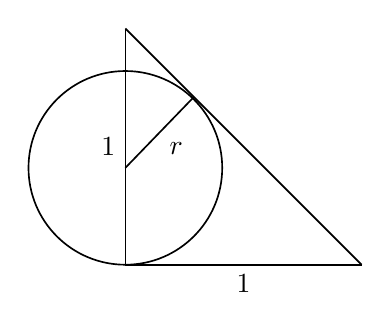
\begin{tikzpicture}[>=stealth, semithick, scale=3]
        \path[draw] (0, 0) -- node[left] {1} (0, 1);
        \path[draw] (0, 0) -- node[below] {1} (1, 0);
        \path[draw] (0, 1) -- (1, 0);
        \draw (0, 0.41) circle (0.41cm);
        \path[draw] (0, 0.41) -- node[below right] {\(r\)} (0.29, 0.71);
    \end{tikzpicture}
    \vspace{0.25cm}
\end{minipage}

Where the circle is tangent to the line containing the hypothenuse of the triangle. What is the value of \(r\)?

It is clear that the circle is centered at \((0, r)\) as it intersects with \((0, 0)\). I will give an analytic solution to this problem. \(r\) is unknown, but let it be fixed. We model the above halfcircle by constructing a function \(f\) from the circle equation in \([0, r]\):
\[
    \sqrt{x^2+(y-r)^2} = r \implies f(x) = \sqrt{r^2-x^2}+r
\]
The hypothenuse can be modelled by the equation \(-x+1\), thus we want to obtain an \(r\) such that there is a single intersection of that curve in this interval:
\[
    \sqrt{r^2-x^2}+r = -x + 1 \implies 0 = x^2 + (r-1)x + \left(-r+\frac{1}{2}\right)
\]
We solve after \(x\):
\[
    x_{1,2} = \frac{1-r}{2} \pm \sqrt{\frac{(r-1)^2}{4}+r-\frac{1}{2}}
\]
For obtaining a single solution, the latter term must be zero. Thus continuing with \(r\):
\[
    \frac{(r-1)^2}{4}+r-\frac{1}{2} = 0 \implies r^2+2r-1=0
\]
Solving for \(r\) obtains two solutions \(-1 \pm \sqrt{2}\), of which only the positive one is of interest. Thus, the solution is \(r = -1 + \sqrt{2}\).

\end{document}
